\section*{Competitions}

\subsection*{Common}

\subsubsection*{Answer a question.} 
Once the contest has started, the user can read the first question. Beneath each question, the user may write his answer in the corresponding input box or he can just select the right answer in case of multiple choice. After answering the question, the user will automatically be brought to the next question. 

\subsubsection*{Navigate between questions.} 
As stated before, when the users answers the current question, he will be brought to the next question. However, during the contest the user will always see the list with all the questions in the question set of the contest. Each question will be presented with his title. Clicking on one of these titles will bring the user to the corresponding question. The user will also be able to go to the next or previous question by clicking on an arrow. 

\subsubsection*{Change answer.} 
The user can change his answer to a specific question. First he navigates to the question as explained before. Then he can see his current answer and if still preferred change his answer. 

\subsubsection*{Remove answer.} 
If the user wants to remove his answer to a specific question, he can press a button that will be positioned next to the answer possibilities. Pressing this button will clean his answer to the question. 

\subsubsection*{See time left.} 
During the contest, the time remaining will be shown. This makes it easy for the users to see how much time they've got left. 

\subsubsection*{Finish a contest.} 
When the user answers the last question, he will not be brought to the next question. Instead, there will be a finish button that the user can click when he wants to finish. After pressing this button, a warning window will appear stating how much time the user got left and asking wether he wants to review his answers or not. He can then press the cancel button to review his answers or press the ok button to finish the contest. Beneath the list of questions, there will also be the same finish button. This makes it easy for the user to finish the contest when he is currently not answering the last question. 

\subsubsection*{See questions that already have been answered.} 
In the list with questions, each question will be marked with some sort of sign to indicate wether the user has already answered this question or not. 

\subsubsection*{See how many points that can be gained or lost.}
Just like the time remaining, the user can always see for each question how many points he can win or lose. This makes it a bit more easy for the user to know the importance of each question. 

\subsubsection*{Example}
An example of how the contest page could look like: 
		\begin{figure}[h]
		  \centering
			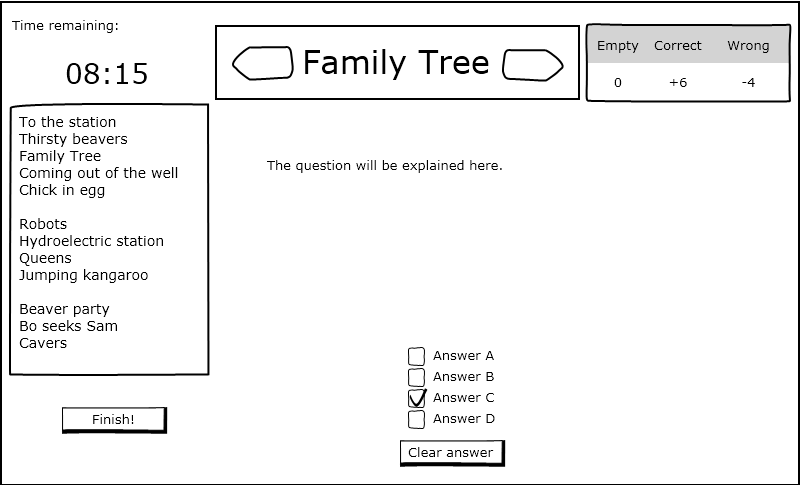
\includegraphics[width=1\textwidth]{img/contests.png}
		  \caption{Contest}
		  \label{Contest}
		\end{figure}

\subsection*{Unrestricted contest}

\subsubsection*{See results and feedback}
Immediatly after finishing the contest, the user will be shown an overview that tells him how well he did on the contest. He can see the list with questions and next to each question he can see his result. Beneath the list with questions, the user can see his total score for the contest. Each question in the list will be clickable. Clicking on one of these will bring the user to the feedback page. On this page the user will be able to reread the question, to see the correct answer together with some sort of explanation and to get more information about this question.  

		\begin{figure}[h]
		  \centering
			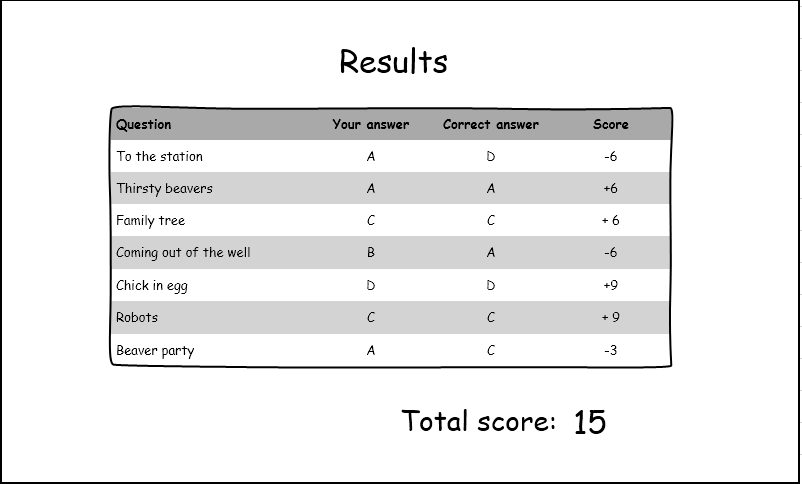
\includegraphics[width=1\textwidth]{img/results.png}
		  \caption{Contest}
		  \label{Contest}
		\end{figure}

\subsection*{Restricted contest}

\subsubsection*{See results and feedback}
After taking a restricted contest, the user can't see his results immediately. The result can be made avaible by the teacher who started the restricted contest. 

\subsection*{Official contest}

\subsubsection*{See results and feedback}
After finishing an official contest, the user will not be able to see his results nor can he see the feedback pages. The user can see his results and the corresponding feedback pages after the official contest has been closed by the organizers. 

